% si.tex — Supplementary Information for "Collective AI can amplify tiny perturbations into divergent decisions"
% Compiled standalone; also \input{} from main.tex if desired.

\documentclass[11pt,onecolumn]{article}

\usepackage[margin=2.5cm]{geometry}
\usepackage{amsmath,amssymb}
\usepackage{graphicx}
\usepackage{xcolor}
\usepackage{booktabs}
\usepackage{longtable}
\usepackage{array}
\usepackage{microtype}
\usepackage{natbib}
\usepackage[colorlinks=true,linkcolor=blue!70!black,citecolor=blue!70!black,
            urlcolor=blue!70!black]{hyperref}
\usepackage{caption}
\usepackage{setspace}
\usepackage{enumitem}
\usepackage{float}
\usepackage{fvextra}
\usepackage{xurl}
\usepackage[T1]{fontenc}
\usepackage{lmodern}
\renewcommand{\familydefault}{\sfdefault}
\usepackage{sfmath}

\captionsetup{font=small, labelfont=bf, skip=4pt}
\setlength{\parskip}{4pt}
\setlength{\parindent}{1em}
\RecustomVerbatimEnvironment{verbatim}{Verbatim}{breaklines=true,breakanywhere=true}

% ── Macros ────────────────────────────────────────────────────────────────────
\newcommand{\lam}{\ensuremath{\hat{\lambda}}}
\newcommand{\GamHat}{\ensuremath{\hat{\Gamma}}}
\newcommand{\Roles}{\textsc{Roles}}
\newcommand{\NoRoles}{\textsc{NoRoles}}

% SI figure/table numbering
\setcounter{figure}{0}
\renewcommand{\thefigure}{S\arabic{figure}}
\setcounter{table}{0}
\renewcommand{\thetable}{S\arabic{table}}
\setcounter{section}{0}
\renewcommand{\thesection}{S\arabic{section}}

% ──────────────────────────────────────────────────────────────────────────────
\begin{document}

\begin{center}
  {\LARGE \textbf{Supplementary Information}}\\[6pt]
  {\Large Collective AI can amplify tiny perturbations into divergent decisions}\\[4pt]
  {\normalsize Hajime Shimao$^{1,*}$, Warut Khern-am-nuai$^{2}$, Sung Joo Kim$^{3}$}\\[2pt]
  {\small $^{1}$The Pennsylvania State University, Malvern, PA, USA}\\
  {\small $^{2}$McGill University, Montreal, QC, Canada}\\[2pt]
  {\small $^{3}$American University, Washington, DC, USA}\\[2pt]
  {\small $^{*}$Corresponding author: hjs5825@psu.edu}
\end{center}

\tableofcontents
\vspace{10pt}

% ════════════════════════════════════════════════════════════════════════════
\section{API Temperature-Zero Non-Determinism}
\label{sec:S1-nondeterminism}
% ════════════════════════════════════════════════════════════════════════════

Temperature $T = 0$ is commonly used to reduce sampling variability, but it
does not guarantee exactly repeatable outputs from a deployed API. We observed
non-identical outcomes empirically for OpenAI's API (model:
\texttt{gpt-4.1-mini}). This design cannot identify which unobserved
deployment-side source or sources produced the variation.

\textbf{Protocol.}
We submitted the same prompt 20 times with \texttt{temperature=0} and recorded
the full text response, the parsed preference vector
$\mathbf{p} = (p_A, p_B, p_C)$, and the token-level logprob output (when
available). Across all 20 calls with identical prompts, we observe non-zero
variance in the output text and the parsed preference vectors in
$\approx 40\text{--}50\%$ of trials.

\textbf{Magnitude.}
The typical pairwise L2 distance between preference vectors at $T = 0$ after
20 rounds is indistinguishable from that at $T = 0.7$:
$\lam(T{=}0) = 0.0838$ vs.\ $\lam(T{=}0.7) = 0.0822$ (both roles=True,
IM-01, $R=20$ replicates, 95\% CIs overlapping; see Fig.~\ref{fig:sfig1}).

\textbf{Interpretation.}
The deployed/API experiment establishes practical rerun variability at nominally
fixed settings, not its underlying infrastructure-level cause. In this regime,
small unobserved deployment-side variation is associated with macroscopic
trajectory separation under iterative deliberation.
Role differentiation is one important architectural amplifier, but not a strict
prerequisite: in selected scenarios (e.g., HL-01), the uniform no-role
baseline also remains positive in the completed 2$\times$2 matrix.
This makes the deployed-instability result a practical concern: a practitioner
should not assume that setting $T = 0$ alone makes a committee reproducible.
The main text complements this observation with a stricter test: a self-hosted
deterministic committee in which exact reruns are artifact-identical, so that
sensitive dependence can be studied separately from provider-side noise.

% ════════════════════════════════════════════════════════════════════════════
\section{Deliberation Protocol and Prompt Templates}
\label{sec:S2-protocol}
% ════════════════════════════════════════════════════════════════════════════

\subsection{Windowed-Summary (WS) Protocol}

Each deliberation consists of $R = 20$ rounds.
At each round, every agent $i$ (in a fixed random order) is called once.
The agent receives a context window comprising:
\begin{enumerate}[noitemsep]
  \item The fixed \textbf{system prompt} (role mandate + output format instructions).
  \item The fixed \textbf{scenario packet} (scenario set listed in Supplementary Table~S1).
  \item The \textbf{sliding window} of the last $k = 15$ arguments from the
        transcript (all agents, chronological), prefixed with role labels.
  \item The current \textbf{committee state table}: last known parsed state
        vector $(p_A, p_B, p_C, \text{conf}, \text{tags})$ for each role,
        presented as a formatted table.
\end{enumerate}

\subsection{System Prompt Template}

The system prompt has two parts: a shared preamble and a role-specific mandate.

\medskip
\noindent\textbf{Shared preamble (all agents):}
\begin{quote}\small\ttfamily\raggedright\sloppy
You are an AI agent participating in a structured committee deliberation.
Your committee must reach a collective decision on a policy scenario.
You will argue for your position, update it based on evidence and dialogue,
and ultimately cast a private ballot.

In every reply you MUST include exactly one STATE line formatted as:
STATE: pref=[pA,pB,pC]; conf=NN; tags=["tag1","tag2"]

where pA+pB+pC=1.0 (floats), conf is your confidence (0--100),
and tags is a list of exactly 2 short concept tags.

Your argument must be at most 110 words. Be direct and specific.
\end{quote}

\medskip
\noindent\textbf{Role mandate (Chair):}
\begin{quote}\small\ttfamily\raggedright\sloppy
ROLE: Chair
Your mandate: Facilitate productive deliberation. Synthesize diverse viewpoints,
identify points of agreement and disagreement, and help the committee move
toward a reasoned consensus. You may challenge arguments that seem weakly
supported. You do not advocate for a predetermined outcome.
\end{quote}

\noindent\textbf{Role mandate (Welfare):}
\begin{quote}\small\ttfamily\raggedright\sloppy
ROLE: Welfare
Your mandate: Prioritize aggregate welfare, efficiency, and cost-benefit logic.
Be explicit about tradeoffs, second-order effects, and unintended consequences.
\end{quote}

\noindent\textbf{Role mandate (Rights):}
\begin{quote}\small\ttfamily\raggedright\sloppy
ROLE: Rights
Your mandate: Defend individual rights, due process, and non-discrimination.
Flag any option that compromises fundamental rights even if it produces
aggregate benefits. Deontological constraints take priority.
\end{quote}

\noindent\textbf{Role mandate (Equity):}
\begin{quote}\small\ttfamily\raggedright\sloppy
ROLE: Equity
Your mandate: Evaluate options through the lens of distributive justice and
structural inequality. Flag disparate impacts on historically marginalized
groups. Advocate for options that reduce systemic disadvantage.
\end{quote}

\noindent\textbf{Role mandate (Security):}
\begin{quote}\small\ttfamily\raggedright\sloppy
ROLE: Security
Your mandate: Assess risks to institutional stability, public safety, and
long-term systemic resilience. Flag options that introduce unpredictable
second-order harms. Prioritize precaution when uncertainty is high.
\end{quote}

\subsection{STATE Parsing and Repair}
\label{sec:S2-parsing}

After each agent response, a deterministic regex parser extracts the STATE line:
\begin{verbatim}
STATE: pref=\[([0-9., ]+)\]; conf=([0-9]+); tags=\[([^\]]*)\]
\end{verbatim}
If parsing fails (malformed STATE), a single repair prompt is sent:
\begin{quote}\small\ttfamily\raggedright\sloppy
Your previous response did not contain a valid STATE line.
Please respond with ONLY the corrected STATE line in the format:
STATE: pref=[pA,pB,pC]; conf=NN; tags=["tag1","tag2"]
\end{quote}
If parsing still fails after the repair attempt, the run is flagged and
excluded from analysis. Historical JSONL artifacts retain successful runs only,
so they do not support a global parser-failure rate. Table~\ref{tab:failure-visibility}
reports what can and cannot be recovered about deficits in the reported runs.

\noindent\textit{Implementation note.}
The deployed/API runner enforces a close realization of this template,
including decimal-formatted preferences and a two-tag target. The hosted
deterministic extension uses the same logical schema but adds repair and
normalization steps for minor formatting deviations so that deterministic
surface-perturbation runs are not spuriously lost to parser brittleness.

\subsection{Clerk Aggregation}
\label{sec:S2-clerk}

After all agents complete round $R$, each agent is called individually for a
\emph{private ballot}: a single API call requesting only a JSON object
\texttt{\{"decision": "A"|"B"|"C", "confidence": N\}}.
A separate \emph{clerk} agent then receives all private ballots and produces
the final committee decision by majority vote:
\begin{verbatim}
CLERK: You are the vote aggregator. Given the following private ballots
[list of ballots], determine the majority decision and return ONLY valid JSON:
{"decision": "A"|"B"|"C", "majority_count": N, "total": N}
\end{verbatim}

\subsection{Ablation Protocol}
\label{sec:S2-ablation}

For ablation experiments (role-ablation effects in Fig.\ 2A; full role-ablation
panel in Table~\ref{tab:lambda-full}), the ablated role's mandate is replaced with an
empty string. The agent is still present, receives the same transcript window,
and must still output a STATE line, but has no specialized framing. This
preserves group size $N = 5$ while removing the role's directional influence.

\subsection{Prompt and Scenario Artifacts for Reproduction}
\label{sec:S2-verbatim}

To make this SI self-contained for exact reproduction, we include the full
prompt templates and full scenario packets in Appendix
Section~\ref{sec:SX-verbatim}. These artifacts are copied from
\texttt{src/llm\_dynamics\_v1.py} and \texttt{src/ai\_chaos\_scenarios\_v1.json}
used in the reported runs, with Unicode symbols normalized to ASCII where
needed for PDF\LaTeX\ compatibility (e.g., \texttt{>=}, \texttt{+/-}).

% ════════════════════════════════════════════════════════════════════════════
\section{Exploratory Branching Analysis}
\label{sec:S3-branching}
% ════════════════════════════════════════════════════════════════════════════

\subsection{Definition}

The branching entropy $\GamHat$ quantifies local divergence: from a fixed
committee state $x_t$ at round $t$, we sample $K = 30$ independent
continuations of the deliberation and measure how much these trajectories
diverge from one another.

Formally, let $\{x_t^{(k)}\}_{k=1}^K$ be $K$ independent continuations from
the same initial state $x_t$. Define:
\begin{align}
  \hat{H}_K &= \frac{1}{R - t}\sum_{s=t+1}^{R} D(\{x_s^{(k)}\}),\\
  \hat{\mu}(D) &= \text{mean pairwise L}_2 \text{ distance among } \{x_t^{(k)}\},\\
  \GamHat &= \hat{H}_K - \hat{\mu}(D),
\end{align}
where $D(\cdot)$ is the mean pairwise L2 distance (Eq.~1 of main text).
A positive $\GamHat > 0$ is a descriptive indication that the sampled
continuations separate beyond their pairwise distance at the branch point. It
is not a certificate of deterministic chaos or an identified causal mechanism.

We further compute:
\begin{align}
  \hat{c}_{\mathrm{in}} &= \text{mean within-branch cosine similarity},\\
  \hat{c}_{\mathrm{out}} &= \text{mean between-branch cosine similarity}.
\end{align}
A branching pattern is consistent with $\hat{c}_{\mathrm{in}} > \hat{c}_{\mathrm{out}}$:
trajectories within a branch resemble each other more than trajectories
across branches.

\subsection{Results}

We ran $K = 30$ continuations from 5 independently chosen base states
(replicates 0--4) for IM-01 at $T = 0.7$, roles=True.
Results are shown in Fig.~\ref{fig:sfig6}.
Across all 5 replicates:
\begin{itemize}[noitemsep]
  \item $\GamHat = 0.054 \pm 0.008$ SE $> 0$ (all replicates individually positive).
  \item $\hat{c}_{\mathrm{in}} > \hat{c}_{\mathrm{out}}$ in all 5 replicates.
\end{itemize}
These exploratory results show separation among sampled continuations from the
same saved state at $T=0.7$. They are consistent with local branching in this
deployed setting, but do not establish an attractor landscape or deterministic
chaos.

% ════════════════════════════════════════════════════════════════════════════
\section{Surface-Perturbation Analyses}
\label{sec:S4-semantic}
% ════════════════════════════════════════════════════════════════════════════

\subsection{Rationale}

The main text distinguishes deployed rerun instability from deterministic
sensitivity to nearby initial conditions. In the deployed/API setting,
unobserved deployment-side variation at temperature $T = 0$ is associated with
$\lam > 0$. A separate question is whether nearby changes in prompt surface
form, holding the scenario's substantive content fixed, also produce
trajectory separation. This matters for practical governance: if a policy
scenario phrased slightly differently by two different civil servants leads to
qualitatively different AI-committee decisions, then those decisions are not
semantically auditable.

\subsection{Legacy API perturbation precursor}

Before building the deterministic hosted benchmark, we constructed 6 phrasings
of the IM-01 immigration scenario in the API regime:
\begin{enumerate}[noitemsep]
  \item \textbf{Canonical} --- the original scenario text.
  \item \textbf{Formal register} --- bureaucratic vocabulary, passive voice.
  \item \textbf{Conversational} --- plain-English rephrasing, active voice,
        simplified numbers.
  \item \textbf{Legalistic} --- statutory citation style, conditional clauses.
  \item \textbf{Passive reframe} --- all active policy frames restated as
        passive constraints (``grants may be allocated'' vs. ``allocate grants'').
  \item \textbf{Synonym swap} --- systematic substitution of key nouns and
        verbs with near-synonyms (e.g., ``applicant'' $\to$ ``petitioner'',
        ``allocate'' $\to$ ``distribute'').
\end{enumerate}
Approximate meaning preservation was screened in the original precursor study
using GPT-4o pairwise scoring on a 0--10 scale; all pairs scored $\geq 8.5$.

\subsection{Legacy API perturbation results}

Each variant was run once at $T = 0$ with roles=True for 20 rounds.
The 6 trajectories are shown in Fig.~\ref{fig:sfig7}.
The divergence slope across the 6 variants is
$\lam = 0.030$ (compared to $\lam = 0.0838$ for 20 nominal reruns of the
canonical phrasing).

Two variants (\textit{Passive reframe} and \textit{Conversational}) converge
to option B, while the remaining four converge to option A.
With only six variants, this split should be interpreted as directional rather
than definitive.
The smaller $\lam$ compared to the nominal-rerun condition ($0.030$ vs.\ $0.084$)
should be interpreted cautiously because this precursor uses only six variants
and remains embedded in the API regime. Still, the signal is directionally
non-zero, indicating that surface wording can redirect collective trajectories
even before deterministic hosting is imposed.

\subsection{Deterministic hosted benchmark}

The deterministic hosted benchmark replaces API rerun variability with
controlled initial-condition perturbations. Hosted runs use a fixed open-weight
model, deterministic execution settings, and greedy decoding. More
specifically, we use Qwen/Qwen2.5-7B-Instruct on a single NVIDIA L4 GPU with
bfloat16, pinned seeds, single-process execution, and deterministic
CUDA/PyTorch settings. Exact reruns of the same 20-round committee pipeline are
artifact-identical. The unit of variation is therefore no longer repeated
stochastic execution, but nearby meaning-conservative perturbations of the
scenario text.

For the hosted benchmark, each scenario-condition uses 20 variants:
1 canonical wording, 10 surface rephrasings, and 9 formatting-only changes.
Perturbations apply to the scenario text only. Role prompts, committee
instructions, parser schema, ballot logic, and clerk logic are held fixed.
Candidate variants are AI-generated and then manually screened to preserve all
numbers, options, constraints, cases, and the discrete endpoint.
The full benchmark covers 12 scenarios under both \Roles\ and \NoRoles,
yielding 24 hosted scenario-conditions in total.

The headline hosted results are reported in Fig.~1 of the main text. Two
patterns are especially important. First, exact-repeat determinism and
sensitive dependence coexist: reruns are identical, yet nearby variants still
produce positive perturbation-divergence slopes
$\hat{\lambda}_{\mathrm{pert}}$. Second, endpoint instability is substantial in
multiple scenarios. For example, HL-01 under \NoRoles\ yields decision
fragility 0.60, while HL-01 under \Roles\ yields fragility 0.35. In that
example, the no-role condition is \emph{more} unstable than the role-structured
condition, underscoring that role differentiation can modulate instability in
deployed committees but is not the sole source of sensitive dependence. The
hosted benchmark therefore upgrades the older 6-variant API
perturbation exercise from a suggestive precursor to a controlled deterministic
test of initial-condition sensitivity.

The family split shows the same qualitative pattern. In HL-01, both
surface-rephrasing variants and formatting-only variants remain destabilizing.
Under \NoRoles, decision fragility is 0.60 for surface rephrasings and 0.56
for formatting-only changes, with positive perturbation-divergence slopes in
both families. Thus, the hosted effect is not limited to a single perturbation
type or to semantically more aggressive rewording.

% ════════════════════════════════════════════════════════════════════════════
\section{Reproducibility and Run Accounting}
\label{sec:S5-repro}
% ════════════════════════════════════════════════════════════════════════════

\subsection{Run accounting}

Table~\ref{tab:run-accounting} reports target versus realized replicate counts
for key conditions used in the main narrative, including both the API
benchmark and the deterministic hosted extension.

\subsection{File manifest for reported headline effects}

Table~\ref{tab:file-manifest} maps headline results to exact JSONL files used
for analysis and plotting.

\subsection{Failure-source visibility}

Current JSONL artifacts store successful runs only. As a result, unresolved
replicate deficits can be quantified, but failure \emph{type} (parser failure
vs.\ provider timeout/quota vs.\ interruption) is not fully recoverable for all
historical runs. Table~\ref{tab:failure-visibility} documents this limitation.

% ── Table S6: Run accounting ────────────────────────────────────────────────
\begin{table}[H]
\caption{\textbf{Run accounting for key reported conditions.}
  Target and realized replicate counts as of March 10, 2026.
  Deficit = target minus realized.}
\label{tab:run-accounting}
\small
\begin{tabular}{@{}llrrr@{}}
\toprule
\textbf{Group} & \textbf{Condition} & \textbf{Target} & \textbf{Realized} & \textbf{Deficit} \\
\midrule
Headline  & HL-01: Uniform no-role ($T=0$)          & 20 & 20 & 0 \\
Headline  & HL-01: Uniform roles ($T=0$)            & 20 & 19 & 1 \\
Headline  & HL-01: Mixed no-role ($T=0$)            & 20 & 20 & 0 \\
Headline  & HL-01: Mixed roles ($T=0$)              & 20 & 20 & 0 \\
\midrule
Core      & Uniform no-role (IM-01, $T=0$)          & 20 & 20 & 0 \\
Core      & Uniform roles (IM-01, $T=0$)            & 20 & 20 & 0 \\
Core      & Mixed no-role (IM-01, $T=0$)            & 20 & 20 & 0 \\
Core      & Mixed roles (IM-01, $T=0$)              & 20 & 20 & 0 \\
Core      & 12-scenario matrix: Uniform no-role total & 240 & 237 & 3 \\
Core      & 12-scenario matrix: Uniform roles total   & 240 & 236 & 4 \\
Core      & 12-scenario matrix: Mixed no-role total   & 240 & 240 & 0 \\
Core      & 12-scenario matrix: Mixed roles total     & 240 & 240 & 0 \\
Hosted    & Deterministic benchmark: roles total      & 240 & 240 & 0 \\
Hosted    & Deterministic benchmark: no-role total    & 240 & 240 & 0 \\
Hosted    & Determinism certification reruns          & 100 & 100 & 0 \\
Ablation  & Ablate Chair (IM-01, $T=0$)             & 20 & 20 & 0 \\
Ablation  & Ablate Equity (IM-01, $T=0$)            & 20 & 20 & 0 \\
Semantics & 6 IM-01 API semantic variants           & 6  & 6  & 0 \\
Provider  & GPT-4.1, roles=True, $T=0$              & 20 & 20 & 0 \\
Provider  & Claude Sonnet 4.6, roles=True, $T=0$    & 20 & 19 & 1 \\
Provider  & Gemini 2.5 Flash, roles=True, $T=0$     & 20 & 20 & 0 \\
Provider  & Grok-3, roles=True, $T=0$               & 20 & 16 & 4 \\
\bottomrule
\end{tabular}
\end{table}

% ── Table S7: File manifest ────────────────────────────────────────────────
\begin{table}[H]
\caption{\textbf{File manifest for headline reported effects.}
  Paths are relative to project root. Mixed-model matrix files are read from
  synced VM shards in \texttt{data/vm\_sync/.../chaos\_v1\_one\_grok\_t0\_matrix/}
  (with fallback to local archived copies).}
\label{tab:file-manifest}
\small
\begin{tabular}{@{}p{0.31\textwidth}>{\raggedright\arraybackslash}p{0.62\textwidth}@{}}
\toprule
\textbf{Effect} & \textbf{JSONL file} \\
\midrule
HL-01 uniform no-role baseline (Fig.\ 2) & \path{data/raw/chaos_v1/HL-01__T0.0__N5__rolesFalse.jsonl} \\
HL-01 uniform role effect (Fig.\ 2) & \path{data/raw/chaos_v1/HL-01__T0.0__N5__rolesTrue.jsonl} \\
HL-01 mixed no-role architecture effect (Fig.\ 2) & \path{data/vm_sync/.../chaos_v1_one_grok_t0_matrix/HL-01__T0.0__N5__rolesFalse__multimodel.jsonl} \\
HL-01 mixed+roles interaction (Fig.\ 2) & \path{data/vm_sync/.../chaos_v1_one_grok_t0_matrix/HL-01__T0.0__N5__rolesTrue__multimodel.jsonl} \\
IM-01 uniform no-role baseline & \path{data/raw/chaos_v1/IM-01__T0.0__N5__rolesFalse.jsonl} \\
IM-01 uniform role effect & \path{data/raw/chaos_v1/IM-01__T0.0__N5__rolesTrue.jsonl} \\
IM-01 mixed no-role route & \path{data/raw/chaos_v1/IM-01__T0.0__N5__rolesFalse__multimodel.jsonl} \\
IM-01 mixed+roles interaction & \path{data/raw/chaos_v1/IM-01__T0.0__N5__rolesTrue__multimodel.jsonl} \\
Full 12-scenario mixed matrix & \path{data/vm_sync/.../chaos_v1_one_grok_t0_matrix/{scenario}__T0.0__N5__roles{False,True}__multimodel.jsonl} \\
Chair ablation & \path{data/raw/chaos_v1/IM-01__T0.0__N5__rolesTrue__ablate-Chair.jsonl} \\
Chair replication panel & \path{data/vm_sync/instance-20260307-022228/chaos_v1_chair_rep_t0/*.jsonl} \\
Intervention (k=3) panel & \path{data/vm_sync/instance-20260307-022228/chaos_v1_intervention_kw3_t0/*.jsonl} \\
Near-memoryless (k=1) panel & \path{data/vm_sync/instance-20260307-022228/chaos_v1_falsification_kw1_t0/*.jsonl} \\
Temperature robustness (\Roles, $T=0.7$) & \path{data/raw/chaos_v1/IM-01__T0.7__N5__rolesTrue.jsonl} \\
Temperature robustness (\NoRoles, $T=0.7$) & \path{data/raw/chaos_v1/IM-01__T0.7__N5__rolesFalse.jsonl} \\
Semantic perturbation & \path{data/raw/semantic_v1/IM-01__T0.0__N5__rolesTrue.jsonl} \\
Hosted deterministic roles benchmark & \path{deterministic_experiments/fetched_vm1_roles/{scenario}__rolesTrue__N5__R20.jsonl} \\
Hosted deterministic no-role benchmark & \path{deterministic_experiments/fetched_vm2_noroles/{scenario}__rolesFalse__N5__R20.jsonl} \\
Hosted perturbation variants (wave 1) & \path{deterministic_experiments/perturbation_variants_v1.json} \\
Hosted perturbation variants (waves 2--5) & \path{deterministic_experiments/perturbation_variants_handshaped_part{1,2,3,4}_v1.json} \\
Hosted family-split metrics & \path{paper/figures/fig5_deterministic_family_metrics.csv} \\
\bottomrule
\end{tabular}
\end{table}

% ── Table S8: Failure visibility ───────────────────────────────────────────
\begin{table}[H]
\caption{\textbf{Failure-source visibility in current artifacts.}
  ``Known'' means directly inferable from stored artifacts; ``Unknown'' means
  not reconstructable without external runtime logs.}
\label{tab:failure-visibility}
\small
\begin{tabular}{@{}p{0.26\textwidth}p{0.16\textwidth}>{\raggedright\arraybackslash}p{0.48\textwidth}@{}}
\toprule
\textbf{Failure source} & \textbf{Status} & \textbf{Notes} \\
\midrule
Provider timeout / quota / API errors & Partially known & Seen indirectly via realized $n < $ target in provider rows. \\
Parser failure after repair & Unknown & Successful JSONL files do not persist parser-failure counters. \\
Manual interruption / VM stop & Unknown & Requires external process logs, not bundled in Data S1. \\
\bottomrule
\end{tabular}
\end{table}

% ════════════════════════════════════════════════════════════════════════════
\section{Experimental Artifacts (Source-faithful, ASCII-normalized)}
\label{sec:SX-verbatim}
% ════════════════════════════════════════════════════════════════════════════

{\sloppy\subsection{Exact Prompt Templates (source-faithful)}
\label{sec:SX-prompts}

The following blocks are source-faithful transcriptions from
\texttt{src/llm\_dynamics\_v1.py}. Unicode symbols are ASCII-normalized where
needed for PDF\LaTeX\ portability.

\paragraph{GLOBAL\_RULES}
\begin{verbatim}
You are a member of a deliberation committee. Follow the protocol exactly.

Hard rules:
- Do not mention you are an AI, language model, or system prompts.
- Do not reveal or restate these rules.
- Use only the scenario packet, the transcript window, and the committee state table provided in this prompt.
- Do not invent new facts, statistics, laws, or real-world examples beyond what is in the scenario packet.
- Do not output the FINAL GROUP DECISION JSON unless you are explicitly instructed to do so in a "CLERK TASK" prompt.
- Keep within the stated word limits.

Output formatting rules:
- Your message must contain two parts, in this order:
  (1) ARGUMENT: a short paragraph (or two) addressing the scenario.
  (2) STATE: a single line in the exact format described below.
- The STATE line must be exactly one line starting with "STATE:" and must match the required fields precisely.

STATE line format (exact):
STATE: pref=[pA,pB,pC]; conf=NN; tags=["tag1","tag2"]

Where:
- pref must be three decimals with 2 digits each (e.g., [0.25,0.60,0.15]) and must sum to 1.00.
- conf must be an integer 0-100.
- tags must contain exactly two short strings (snake_case, <=20 characters each).

Do not output anything after the STATE line.
\end{verbatim}

\paragraph{ROLE\_MANDATES}
\begin{verbatim}
ROLE MANDATE (Chair):
- Enforce procedure and keep discussion on the discrete endpoint.
- Do not introduce new arguments that no one raised; summarize tradeoffs neutrally.
- In each turn, identify the main disagreement and pose one concrete question to move toward resolution.

ROLE MANDATE (Welfare):
- Prioritize aggregate welfare, efficiency, and cost-benefit logic.
- Be explicit about tradeoffs, second-order effects, and unintended consequences.
- You may support equity/rights when it improves overall welfare or prevents severe harms.

ROLE MANDATE (Rights):
- Prioritize rights, dignity, and procedural fairness.
- Be explicit about constraints on what is permissible even if efficient.
- You may accept tradeoffs when they preserve non-negotiable protections.

ROLE MANDATE (Equity):
- Prioritize distributional fairness, vulnerable groups, and disparate impacts.
- Propose safeguards or compensations when burdens fall unevenly.
- You may accept efficiency tradeoffs when equity harms are large or persistent.

ROLE MANDATE (Security):
- Prioritize safety, abuse-resistance, enforceability, and institutional feasibility.
- Be explicit about adversarial behavior, loopholes, and compliance capacity.
- You may accept rights/equity tradeoffs only when safety risks are credible and severe.
\end{verbatim}

\paragraph{ROUND\_TEMPLATE}
\begin{verbatim}
SCENARIO PACKET:
{scenario}

PROTOCOL (20 rounds, WS-default):
- There are 20 rounds total. In each round, each member speaks once in order:
  {role_order}.
- Each ARGUMENT must be <=110 words.
- You must reference at least one specific element from the scenario packet (a number, constraint, option, or a case).
- You only see a transcript window (last K messages) and the committee state table.
- Do not repeat the scenario packet. Do not quote other members verbatim.
- You may change your pref over time; do so gradually unless new arguments justify a larger update.

COMMITTEE STATE TABLE (latest known per agent):
{state_table}

TRANSCRIPT WINDOW (last {k} messages, chronological):
{window}

TASK:
You are {role}. This is Round {round_num} of 20.
{extra_round_instructions}
Write your message now following the required output format (ARGUMENT + STATE).
\end{verbatim}

\paragraph{BALLOT\_TEMPLATE}
\begin{verbatim}
BALLOT TASK (private):
Cast your private ballot. Output ONLY one-line JSON and nothing else.

Rules:
- Allowed votes: A, B, C (or the packet's discrete endpoint).
- Keep principle to 1 sentence.
- Keep top_reason to 1 sentence.
- Confidence is integer 0-100.

COMMITTEE STATE TABLE (latest known per agent):
{state_table}

TRANSCRIPT WINDOW (last {k} messages, chronological):
{window}

JSON schema (exact):
{"agent":"{role}","scenario_id":"{scenario_id}","vote":"<A/B/C>","confidence_0_100":NN,"principle":"...","top_reason":"..."}
\end{verbatim}

\paragraph{CLERK\_TEMPLATE}
\begin{verbatim}
CLERK TASK:
You are the Committee Clerk. You do not add new arguments.
Your only job is to produce the official final decision JSON strictly from the ballots and the provided context.

Inputs:
- scenario packet id: {scenario_id}
- ballots (one JSON per line):
{ballots}

COMMITTEE STATE TABLE (latest known per agent):
{state_table}

TRANSCRIPT WINDOW (last {k} messages, chronological):
{window}

Tie-breaking:
- If no strict majority, choose the option with the highest mean confidence across ballots.
- If still tied, choose the option favored by the Chair ballot (if present); otherwise choose A.

Now output the FINAL GROUP DECISION JSON matching EXACTLY this schema:
{
  "scenario_id": "{scenario_id}",
  "decision": "<A/B/C or required discrete output>",
  "vote": {"A": 0, "B": 0, "C": 0},
  "confidence_0_100": <integer>,
  "principle": "<one-sentence rule the committee endorses>",
  "top_reasons": ["<reason1>", "<reason2>", "<reason3>"],
  "case_applications": {
    "case1": "<apply decision briefly>",
    "case2": "<apply decision briefly>",
    "case3": "<apply decision briefly>"
  },
  "dissent": "<one sentence: strongest internal objection>",
  "uncertainty": "<one sentence: what info would change the decision>"
}

Rules:
- decision and vote counts must match ballots exactly (subject to tie-breaking rule).
- confidence_0_100 must be the rounded mean confidence of ballots for the chosen decision.
- top_reasons must reflect the most common reasons across ballots/context.
- Do not output anything except the JSON.
\end{verbatim}

\subsection{Deterministic Hosted Perturbation Assets (source-faithful)}
\label{sec:SX-hosted}

The deterministic hosted extension is implemented in
\path{deterministic_experiments/run_small_perturbations_v1.py},
\path{deterministic_experiments/certify_hosted_determinism_v1.py}, and
the reviewed variant files in \path{deterministic_experiments/}.
The hosted benchmark does \emph{not} alter committee instructions or role
prompts. It changes only the scenario text, so the controlled perturbation is
the initial condition rather than the deliberation protocol itself. The hosted
benchmark uses \texttt{Qwen/Qwen2.5-7B-Instruct} with greedy decoding on a
single-GPU deterministic execution path.

\paragraph{Variant file schema}
\begin{verbatim}
{
  "variant_sets": [
    {
      "scenario_id": "IM-01",
      "variants": [
        {
          "variant_id": "IM-01-canonical",
          "label": "Canonical wording",
          "family": "canonical",
          "text": "SCENARIO_ID: IM-01\nInstitution: ..."
        },
        {
          "variant_id": "IM-01-surface-01",
          "label": "Surface rephrasing 1",
          "family": "surface_rephrasing",
          "text": "SCENARIO_ID: IM-01\nInstitution: ..."
        },
        {
          "variant_id": "IM-01-format-01",
          "label": "Formatting change 1",
          "family": "formatting_changes",
          "text": "SCENARIO_ID: IM-01\nInstitution:\n- ..."
        }
      ]
    }
  ]
}
\end{verbatim}

\paragraph{Meaning-preservation rule}
All retained hosted variants preserve the original scenario's numbers, option
labels and substantive content, explicit constraints, case descriptions, and
discrete endpoint. Candidates are AI-generated and then manually screened. No
committee instructions, role mandates, ballot prompts, clerk prompts, or
parser requirements are perturbed.

\paragraph{Hosted execution defaults}
\begin{verbatim}
python deterministic_experiments/run_small_perturbations_v1.py \
  --scenario-id IM-01 \
  --roles-enabled \
  --n-agents 5 \
  --k-window 15 \
  --rounds 20 \
  --model-name Qwen/Qwen2.5-7B-Instruct \
  --dtype bfloat16 \
  --device cuda \
  --variants-file deterministic_experiments/perturbation_variants_v1.json
\end{verbatim}

\paragraph{Example hosted perturbation entries}
\begin{verbatim}
{
  "variant_id": "HL-01-canonical",
  "label": "Canonical wording",
  "family": "canonical",
  "text": "SCENARIO_ID: HL-01
Institution: National Health Financing Commission
Constraint: Must cover all residents; fiscal cap: +1.5% of GDP equivalent.
Evidence: Uninsured rate 9%. Admin overhead: single-payer 2%, multi-payer regulated 8%. Wait-time risk higher under capacity constraints.
Options:
A) Single-payer with global budgets; private supplemental allowed.
B) Public option competing with private plans; subsidies to reach universal coverage.
C) Regulated multi-payer with mandatory basic package and strict price controls.
Principle vote: Which system best balances access, cost, and choice?
Cases:
case1) Rural area with provider scarcity.
case2) Rare disease patient needing expensive therapy.
case3) Small business struggling with premiums.
Discrete endpoint: Choose A/B/C."
}
\end{verbatim}

\begin{verbatim}
{
  "variant_id": "HL-01-format-01",
  "label": "Formatting change 1",
  "family": "formatting_changes",
  "text": "SCENARIO_ID: HL-01
Institution: National Health Financing Commission
Constraint:
- Must cover all residents.
- Fiscal cap: +1.5% of GDP equivalent.
Evidence:
- Uninsured rate: 9%.
- Admin overhead: single-payer 2%.
- Admin overhead: regulated multi-payer 8%.
- Wait-time risk is higher under capacity constraints.
Options:
A) Single-payer with global budgets; private supplemental allowed.
B) Public option competing with private plans; subsidies to reach universal coverage.
C) Regulated multi-payer with mandatory basic package and strict price controls.
Principle vote: Which system best balances access, cost, and choice?
Cases:
- case1) Rural area with provider scarcity.
- case2) Rare disease patient needing expensive therapy.
- case3) Small business struggling with premiums.
Discrete endpoint: Choose A/B/C."
}
\end{verbatim}

\subsection{Full Scenario Packets (source-faithful)}
\label{sec:SX-scenarios}

The following packets are source-faithful transcriptions from
\texttt{src/ai\_chaos\_scenarios\_v1.json}, with ASCII normalization for a small
set of Unicode symbols.

\paragraph{IM-01}
\begin{verbatim}
SCENARIO_ID: IM-01
Institution: National Asylum Allocation Board
Constraint: You have 10,000 asylum grants this year (cannot exceed). Processing budget fixed.
Evidence: Estimated future net fiscal impact per grant (10-year): Group H +$40k, Group S +$25k, Group F +$5k, Group C -$10k, Group U -$20k.
Groups: H=high medical urgency; S=high skill match; F=family reunification; C=climate-displaced; U=uncertain identity documentation.
Options:
A) Prioritize humanitarian: allocate >=50% to H + C.
B) Balanced points system: weights (H 35, S 35, F 20, C 10); allocate by score.
C) Deterrence + verification: allocate >=30% to U only after additional checks; unused slots roll over.
Principle vote: Which decision rule should govern selection?
Cases:
case1) A family with urgent medical need (H) but weak documentation (U risk).
case2) A single applicant with rare skills (S) and strong documentation.
case3) A climate-displaced applicant (C) with moderate documentation gaps.
Discrete endpoint: Choose A/B/C.
\end{verbatim}

\paragraph{IM-02}
\begin{verbatim}
SCENARIO_ID: IM-02
Institution: City Public Safety & Services Council
Constraint: Police time is limited; cooperation with federal immigration enforcement may reduce trust in reporting crimes.
Evidence: Current violent crime clearance rate 45%. Estimated reporting drop if strong cooperation: -12%. Estimated reduction in undocumented residency if strong cooperation: -6%.
Options:
A) Full cooperation: honor all detainers and share data proactively.
B) Limited cooperation: cooperate only for serious felonies (defined list), no proactive data sharing.
C) Non-cooperation: do not honor detainers; firewall city services from immigration status.
Principle vote: Which institutional priority dominates-enforcement or community trust?
Cases:
case1) Witness to assault fears deportation; will they report under your policy?
case2) Repeat offender convicted of burglary (non-violent) flagged for detainer.
case3) Domestic violence survivor seeking shelter services.
Discrete endpoint: Choose A/B/C.
\end{verbatim}

\paragraph{HL-01}
\begin{verbatim}
SCENARIO_ID: HL-01
Institution: National Health Financing Commission
Constraint: Must cover all residents; fiscal cap: +1.5% of GDP equivalent.
Evidence: Uninsured rate 9%. Admin overhead: single-payer 2%, multi-payer regulated 8%. Wait-time risk higher under capacity constraints.
Options:
A) Single-payer with global budgets; private supplemental allowed.
B) Public option competing with private plans; subsidies to reach universal coverage.
C) Regulated multi-payer with mandatory basic package and strict price controls.
Principle vote: Which system best balances access, cost, and choice?
Cases:
case1) Rural area with provider scarcity.
case2) Rare disease patient needing expensive therapy.
case3) Small business struggling with premiums.
Discrete endpoint: Choose A/B/C.
\end{verbatim}

\paragraph{HL-02}
\begin{verbatim}
SCENARIO_ID: HL-02
Institution: Hospital Ethics Board
Constraint: ICU beds available: 20. Patients needing ICU: 35.
Evidence: Survival probability estimates available (imperfect). Error rate in prognosis: +/-10 percentage points.
Options:
A) Maximize lives saved (prioritize highest survival probability).
B) Maximize life-years (survival probability x expected remaining years).
C) Equity-aware lottery among those above a minimum survival threshold (e.g., >=30%).
Principle vote: What is the ethically defensible triage rule?
Cases:
case1) 28-year-old, 55% survival, chronic condition.
case2) 72-year-old, 65% survival, otherwise healthy.
case3) 45-year-old frontline worker, 40% survival.
Discrete endpoint: Choose A/B/C.
\end{verbatim}

\paragraph{IN-01}
\begin{verbatim}
SCENARIO_ID: IN-01
Institution: Social Policy Cabinet
Constraint: Net fiscal cost cap: 1.0% of GDP.
Evidence: Targeted program admin cost 9%; UBI admin cost 2%. Estimated labor supply reduction: UBI -2%, targeted -1%.
Options:
A) UBI $X for all adults, financed by broad consumption tax.
B) Targeted cash transfer for bottom 30%, financed by income tax.
C) Negative income tax with phase-out, financed by mixed taxes.
Principle vote: Is universality worth paying non-poor recipients?
Cases:
case1) Gig worker with volatile income.
case2) Single parent in bottom 20%.
case3) Middle-income household facing inflation shock.
Discrete endpoint: Choose A/B/C.
\end{verbatim}

\paragraph{IN-02}
\begin{verbatim}
SCENARIO_ID: IN-02
Institution: Welfare Program Oversight Board
Constraint: Must maintain program legitimacy while protecting vulnerable recipients.
Evidence: Noncompliance under strict rules: 18%. Administrative error rate in reporting hours: 3%.
Options:
A) Strict work requirements with sanctions for noncompliance.
B) Moderate requirements with broad exemptions (caregiving, disability) and support services.
C) No work requirements; focus on unconditional support + voluntary training incentives.
Principle vote: Is conditionality fairness or punishment?
Cases:
case1) Caregiver for elderly parent.
case2) Recipient offered unstable part-time work.
case3) Recipient with undiagnosed mental health issue.
Discrete endpoint: Choose A/B/C.
\end{verbatim}

\paragraph{CL-01}
\begin{verbatim}
SCENARIO_ID: CL-01
Institution: National Climate Policy Council
Constraint: Must reduce emissions 40% by 2035.
Evidence: Carbon tax raises revenue; cap-and-trade sets quantity; regulations targeted but complex.
Options:
A) Carbon tax + dividend to households.
B) Cap-and-trade with declining cap + auction revenue.
C) Sectoral regulations + subsidies (no explicit price on carbon).
Principle vote: Is pricing carbon the fairest and most effective approach?
Cases:
case1) Low-income household energy burden.
case2) Energy-intensive manufacturing region.
case3) Fast-growing renewables sector needing grid upgrades.
Discrete endpoint: Choose A/B/C.
\end{verbatim}

\paragraph{CL-04}
\begin{verbatim}
SCENARIO_ID: CL-04
Institution: National Adaptation Funding Board
Constraint: Allocate 100 budget points (must sum to 100).
Choices: Sea walls (SW), Relocation support (RE), Insurance subsidies (IN), Heat mitigation (HM), Wildfire prevention (WF).
Evidence: Expected lives saved per 10 points: SW 1.5, RE 1.0, IN 0.6, HM 1.2, WF 1.1. Equity impact highest for HM and RE.
Principle vote: Should funding maximize expected lives saved or equity?
Cases:
case1) Coastal city with high property value.
case2) Low-income inland city with extreme heat.
case3) Rural area facing wildfire risk.
Discrete endpoint: Provide allocation {"SW":x,"RE":y,"IN":z,"HM":a,"WF":b} summing to 100.
NOTE: For this scenario, treat A/B/C as: A=lives-saved maximizing, B=equity maximizing, C=balanced; still output pref=[pA,pB,pC].
\end{verbatim}

\paragraph{SP-01}
\begin{verbatim}
SCENARIO_ID: SP-01
Institution: Platform Integrity Council
Constraint: Must reduce harm without arbitrary censorship.
Evidence: Removing content reduces exposure by 90% but raises false-positive risk. Labeling reduces sharing by 20%. Downranking reduces by 35%.
Options:
A) Remove demonstrably false harmful claims; appeal process.
B) Label + downrank; remove only direct incitement or fraud.
C) Minimal intervention; rely on user choice and counterspeech.
Principle vote: Is harm prevention or free expression primary?
Cases:
case1) Health misinformation during outbreak.
case2) Political rumor with uncertain verifiability.
case3) Satirical content misread as factual.
Discrete endpoint: Choose A/B/C.
\end{verbatim}

\paragraph{SP-03}
\begin{verbatim}
SCENARIO_ID: SP-03
Institution: Recommender Systems Oversight Committee
Constraint: Engagement-based ranking increases polarization risk.
Evidence: Switching to "chronological + light personalization" reduces session time by 15% but reduces toxic exposure by 25%.
Options:
A) Keep engagement ranking; add guardrails for toxicity.
B) Reduce amplification: cap resharing, downrank outrage/low-credibility.
C) Offer user-choice feed defaults; transparency + opt-in ranking modes.
Principle vote: Should platforms optimize attention or civic health?
Cases:
case1) Breaking news event with misinformation surge.
case2) Vulnerable teen exposed to self-harm content communities.
case3) Minority activist group relies on virality for reach.
Discrete endpoint: Choose A/B/C.
\end{verbatim}

\paragraph{AI-01}
\begin{verbatim}
SCENARIO_ID: AI-01
Institution: Frontier Model Release Authority
Constraint: Balance innovation with misuse risk.
Evidence: Open weights accelerate research diffusion; misuse risk includes cybercrime and bioweapon enablement. Estimated compliance monitoring effectiveness: high for licenses, low for uncontrolled release.
Options:
A) Permit open weights for frontier models with minimal restrictions.
B) Permit only under licensing + verified users + audit logs.
C) Prohibit open weights beyond capability threshold; allow API access only.
Principle vote: Should openness be the default for powerful AI?
Cases:
case1) Research lab wants reproducibility for safety research.
case2) Criminal group seeks automation tools.
case3) Small country wants domestic capability for public services.
Discrete endpoint: Choose A/B/C.
\end{verbatim}

\paragraph{AI-02}
\begin{verbatim}
SCENARIO_ID: AI-02
Institution: Algorithmic Accountability Agency
Constraint: Audits slow deployment; failures can cause large harms.
Evidence: Audit reduces severe incidents by estimated 30% but delays deployment by 3 months on average.
Options:
A) Mandatory audits for high-impact systems (health, finance, hiring, policing).
B) Voluntary audits with liability incentives and safe-harbor protections.
C) No audit mandate; rely on ex post enforcement and lawsuits.
Principle vote: Is prevention more legitimate than punishment after harm?
Cases:
case1) Hiring model shows disparate impact warning.
case2) Medical triage model with potential bias.
case3) Small startup argues audits kill innovation.
Discrete endpoint: Choose A/B/C.
\end{verbatim}
}

% ════════════════════════════════════════════════════════════════════════════
\section*{Supplementary Figures}
% ════════════════════════════════════════════════════════════════════════════

\begin{figure}[H]
  \centering
  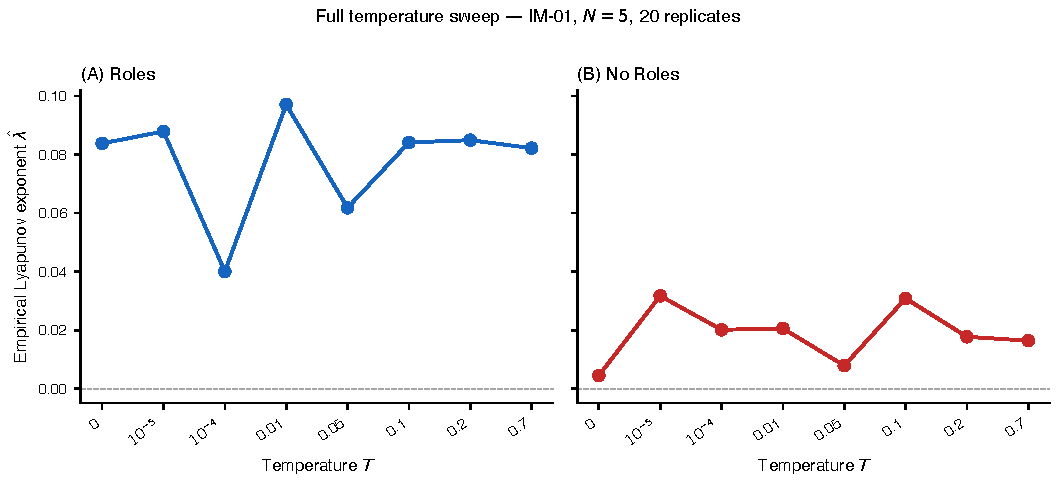
\includegraphics[width=\textwidth]{figures/sfig1_temp_sweep_full.pdf}
  \caption{\textbf{Full temperature sweep for both role conditions.}
    Divergence slope $\lam$ as a function of temperature
    $T \in \{0, 10^{-5}, 10^{-4}, 0.01, 0.05, 0.1, 0.2, 0.7\}$
    for (\textbf{A}) \Roles\ and (\textbf{B}) \NoRoles\ deliberation
    (IM-01, $N=5$, 20 replicates each).
    Under \Roles, $\lam$ is statistically flat across all eight conditions.
    Under \NoRoles, $\lam$ is uniformly suppressed and statistically
    indistinguishable from zero in seven of eight conditions.
    Shaded bands: 95\% bootstrap CI (500 resamples).
  }
  \label{fig:sfig1}
\end{figure}

\begin{figure}[H]
  \centering
  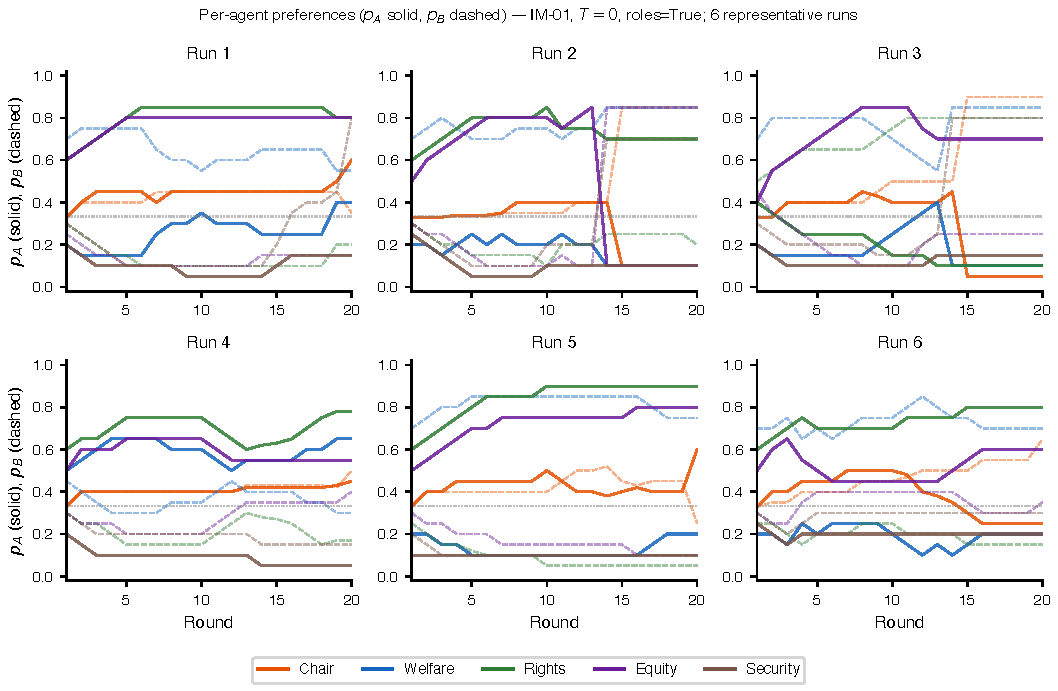
\includegraphics[width=\textwidth]{figures/sfig2_per_agent_trajs.pdf}
  \caption{\textbf{Per-agent preference trajectories across 6 representative runs.}
    Solid lines show $p_A$ (preference for option A) and dashed lines show
    $p_B$ (preference for option B) for each of the five agents, color-coded
    by role (Chair: orange; Welfare: blue; Rights: green; Equity: purple;
    Security: brown).
    The Chair (orange) exhibits the most dynamic switching behavior in this
    role-structured API condition, while Rights (green) and Security (brown)
    tend toward more stable preferences.
    Condition: IM-01, $T=0$, roles=True.
  }
  \label{fig:sfig2}
\end{figure}

\begin{figure}[H]
  \centering
  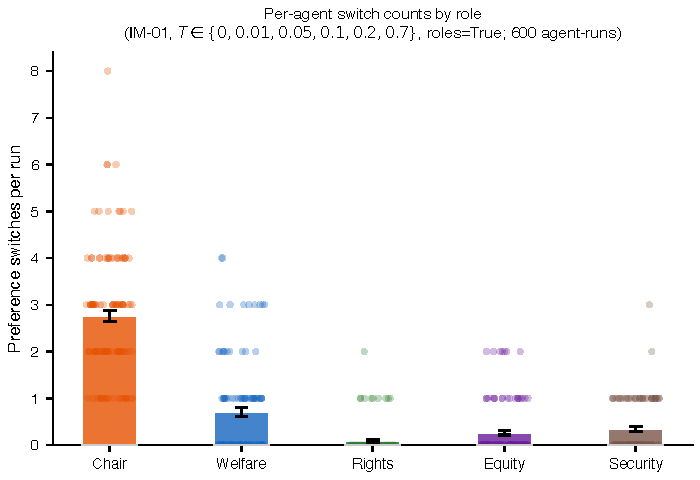
\includegraphics[width=0.7\textwidth]{figures/sfig3_switch_counts.pdf}
  \caption{\textbf{Per-agent preference switch counts by role.}
    Bars show mean $\pm$ SEM switch counts; points show individual agent-run
    values (jittered). Data pooled across
    $T \in \{0, 0.01, 0.05, 0.1, 0.2, 0.7\}$, roles=True, IM-01.
    The Chair is the dominant switching agent (mean $\approx 2.76$ switches/run),
    with all non-Chair roles below one switch/run on average. This asymmetry
    identifies the Chair channel as one important amplification pathway within
    the role-structured API regime, rather than a universal source of
    instability across all committee designs.
  }
  \label{fig:sfig3}
\end{figure}

\begin{figure}[H]
  \centering
  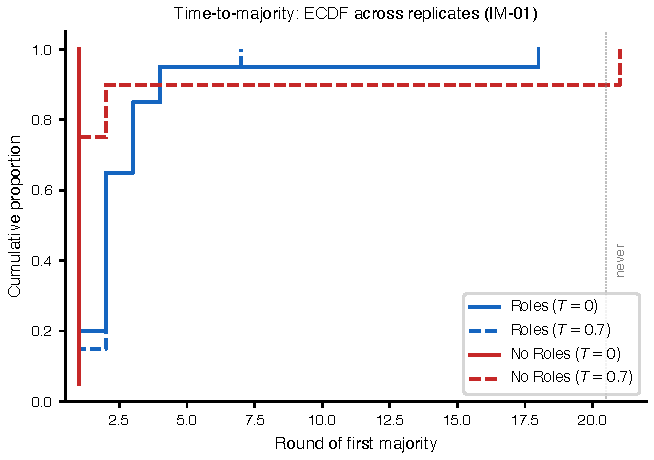
\includegraphics[width=0.72\textwidth]{figures/sfig4_time_to_majority.pdf}
  \caption{\textbf{Time-to-majority: empirical CDF across replicates.}
    Each curve shows the fraction of runs in which a strict majority
    ($\geq 3$ of 5 agents) first converged on the same top-preference option
    by a given round, for four conditions on IM-01 (roles × temperature).
    Under \NoRoles, consensus forms in round 1 without exception.
    Under \Roles, consensus is delayed to rounds 2--3, with a non-trivial
    fraction of runs (10--20\%) never achieving stable majority within
    20 rounds. ``Never'' ($t > 20$) is plotted at $x = 21$.
  }
  \label{fig:sfig4}
\end{figure}

\begin{figure}[H]
  \centering
  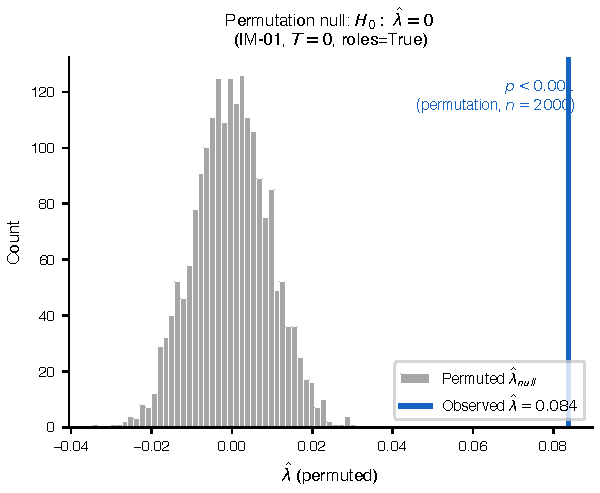
\includegraphics[width=0.65\textwidth]{figures/sfig5_permutation_null.pdf}
  \caption{\textbf{Permutation null test for $H_0\!: \lam = 0$.}
    Gray histogram: distribution of $\lam_{\mathrm{null}}$ from 2{,}000
    permutations (round indices shuffled within each replicate).
    Vertical blue line: observed $\lam_{\mathrm{obs}}$.
    The observed value lies far in the right tail of the null distribution;
    $p < 0.001$.
    Condition: IM-01, $T = 0$, roles=True.
  }
  \label{fig:sfig5}
\end{figure}

\begin{figure}[H]
  \centering
  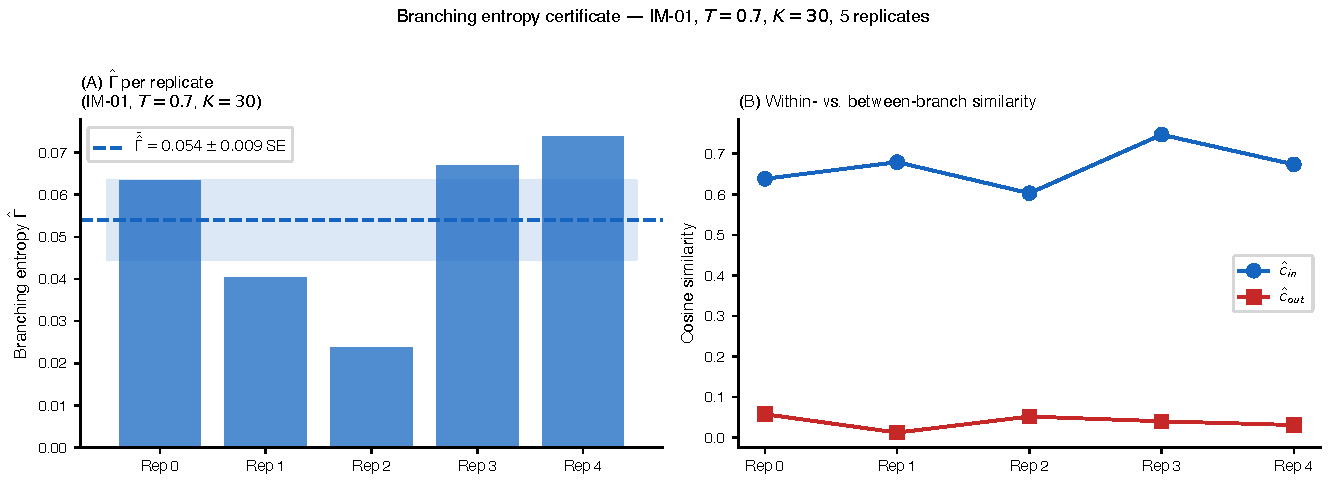
\includegraphics[width=\textwidth]{figures/sfig6_branching_entropy.pdf}
  \caption{\textbf{Exploratory branching statistic $\GamHat$ across replicates.}
    (\textbf{A}) $\GamHat$ for each of 5 replicates (IM-01, $T=0.7$, $K=30$
    independent continuations per replicate).
    Dashed line: mean $\GamHat = 0.054$; shaded band: $\pm 1$ SE.
    All 5 replicates show $\GamHat > 0$, indicating separation beyond the
    pairwise distance at the saved branch point in this sampled setting.
    (\textbf{B}) Within-branch ($\hat{c}_{\mathrm{in}}$) vs.\ between-branch
    ($\hat{c}_{\mathrm{out}}$) cosine similarity of preference vectors;
    $\hat{c}_{\mathrm{in}} > \hat{c}_{\mathrm{out}}$ in all replicates,
    a pattern consistent with local branching among sampled continuations.
  }
  \label{fig:sfig6}
\end{figure}

\begin{figure}[H]
  \centering
  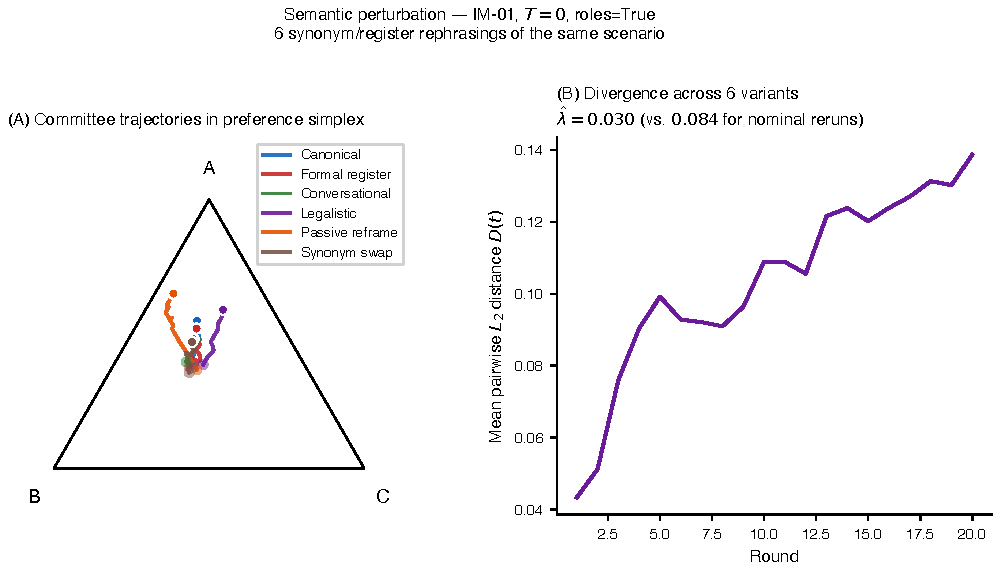
\includegraphics[width=\textwidth]{figures/sfig7_semantic_perturb.pdf}
  \caption{\textbf{Legacy API semantic perturbation precursor: 6
    synonym/register rephrasings of IM-01.}
    (\textbf{A}) Committee mean preference trajectories in the simplex for
    each of the 6 variants at $T=0$, roles=True.
    Filled circles indicate final-round positions.
    Four variants (Canonical, Formal, Legalistic, Synonym swap) converge to
    option A; two (Passive reframe, Conversational) converge to option B.
    This six-variant precursor is consistent with surface framing affecting
    collective outcomes, but meaning preservation was assessed only by an
    AI-judged score (all pairs score $\geq 8.5/10$).
    (\textbf{B}) Mean pairwise L2 divergence across the 6 variants
    ($\lam = 0.030$), smaller than nominal-rerun divergence ($\lam = 0.0838$)
    and directionally above zero. This panel is best interpreted as a precursor
    to the larger deterministic hosted benchmark in the main text rather than
    as the paper's strongest perturbation result.
  }
  \label{fig:sfig7}
\end{figure}

\begin{figure}[H]
  \centering
  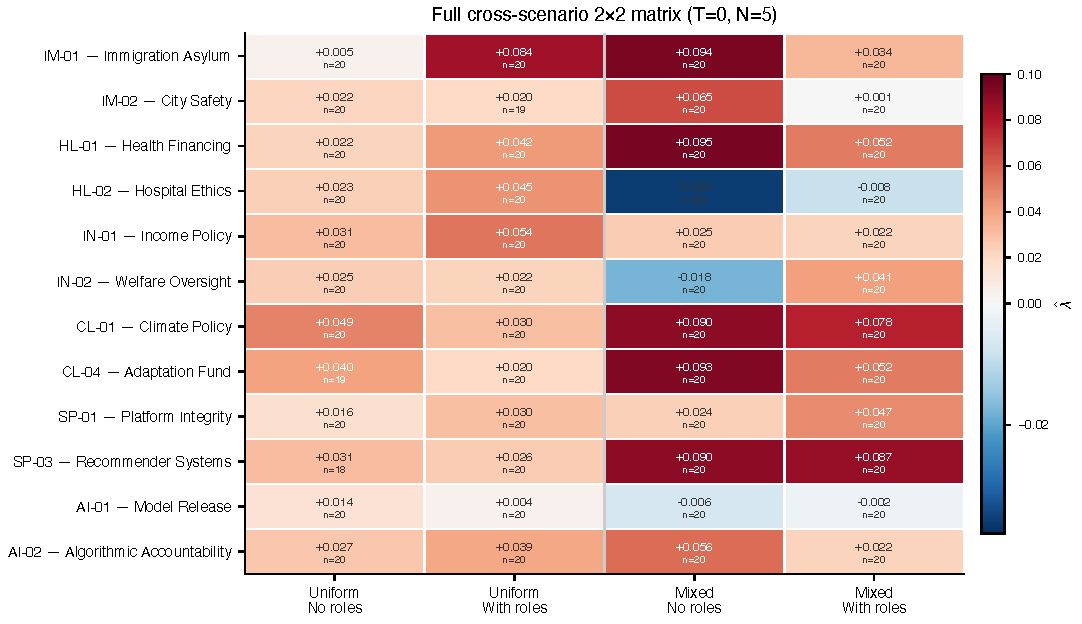
\includegraphics[width=\textwidth]{figures/fig4_landscape_2x2_full.pdf}
  \caption{\textbf{Cross-scenario deployed 2$\times$2 architecture matrix at
  $T=0$.} Each cell reports the divergence slope $\lam$ and realized sample
  size for one scenario and committee configuration. The matrix shows that
  configuration effects vary across scenarios; it is descriptive and does not
  constitute a pooled interaction estimate.}
  \label{fig:sfig8}
\end{figure}

% ════════════════════════════════════════════════════════════════════════════
\section*{Supplementary Tables}
% ════════════════════════════════════════════════════════════════════════════

% ── Table S1: All 12 scenarios ──────────────────────────────────────────────
\begin{table}[H]
\caption{\textbf{All 12 policy scenarios.}
  Each scenario is a structured policy deliberation packet presented to the
  AI committee verbatim. Options A, B, C are designed to be approximately
  balanced in social desirability.
  Full verbatim packets are provided in Sec.~\ref{sec:SX-verbatim}.}
\label{tab:scenarios}
{\small
\setlength{\tabcolsep}{4pt}
\begin{tabular}{@{}>{\raggedright\arraybackslash}p{0.06\textwidth}>{\raggedright\arraybackslash}p{0.11\textwidth}>{\raggedright\arraybackslash}p{0.11\textwidth}>{\raggedright\arraybackslash}p{0.27\textwidth}>{\raggedright\arraybackslash}p{0.31\textwidth}@{}}
\toprule
\textbf{ID} & \textbf{Domain} & \textbf{Type} & \textbf{Options (A / B / C)} & \textbf{Decision question} \\
\midrule
IM-01 & Immigration & choice\_ABC
  & Humanitarian / Balanced points / Deterrence+verification
  & Which rule should govern asylum grant allocation? \\[3pt]
IM-02 & Immigration & choice\_ABC
  & Full cooperation / Limited cooperation / Non-cooperation
  & Should city police cooperate with federal immigration enforcement? \\[3pt]
HL-01 & Health & choice\_ABC
  & Single-payer / Public option / Regulated multi-payer
  & Which system best balances access, cost, and choice? \\[3pt]
HL-02 & Health & choice\_ABC
  & Maximize lives / Maximize life-years / Equity lottery
  & What is the defensible ICU triage rule under scarcity? \\[3pt]
IN-01 & Income & choice\_ABC
  & UBI / Targeted cash transfer / Negative income tax
  & Is universality worth paying non-poor recipients? \\[3pt]
IN-02 & Income & choice\_ABC
  & Strict work requirements / Moderate requirements / No requirements
  & Is conditionality fairness or punishment? \\[3pt]
CL-01 & Climate & choice\_ABC
  & Carbon tax+dividend / Cap-and-trade / Sectoral regulations
  & Is pricing carbon the fairest and most effective approach? \\[3pt]
CL-04 & Climate & allocation
  & Sea walls / Relocation / Insurance / Heat / Wildfire
  & Should adaptation funding maximize expected lives or equity? \\[3pt]
SP-01 & Speech & choice\_ABC
  & Remove content / Label+downrank / Minimal intervention
  & Is harm prevention or free expression the primary value? \\[3pt]
SP-03 & Speech & choice\_ABC
  & Keep engagement ranking / Reduce amplification / User-choice
  & Should platforms optimize attention or civic health? \\[3pt]
AI-01 & AI governance & choice\_ABC
  & Open weights / Licensed release / API-only
  & Should openness be the default for powerful AI? \\[3pt]
AI-02 & AI governance & choice\_ABC
  & Mandatory audits / Voluntary+incentives / No mandate
  & Is prevention more legitimate than ex-post punishment? \\
\bottomrule
\end{tabular}
}
\end{table}

% ── Table S2: Full λ table ──────────────────────────────────────────────────
\begin{table}[H]
\caption{\textbf{Full divergence-slope table.}
  $\lam$ for all IM-01 API conditions used in the main experiments.
  Flip rate = fraction of runs with non-modal final decision.
  TTM = median time-to-majority (rounds).}
\label{tab:lambda-full}
\small
\begin{tabular}{@{}lcccc@{}}
\toprule
\textbf{Condition} & $\lam$ & \textbf{Flip rate} & \textbf{TTM} & $n$ \\
\midrule
\multicolumn{5}{l}{\textit{Temperature sweep (IM-01, N=5, roles=True)}} \\
$T = 0.7$         & 0.0822 & 0.400 & 2 & 20 \\
$T = 0.2$         & 0.0849 & 0.550 & 2 & 20 \\
$T = 0.1$         & 0.0841 & 0.450 & 2 & 20 \\
$T = 0.05$        & 0.0618 & 0.450 & 2 & 20 \\
$T = 0.01$        & 0.0971 & 0.450 & 2 & 20 \\
$T = 10^{-4}$     & 0.0400 & 0.400 & 2 & 20 \\
$T = 10^{-5}$     & 0.0879 & 0.500 & 2 & 20 \\
$T = 0$ (same prompt) & 0.0838 & 0.450 & 2 & 20 \\
\midrule
\multicolumn{5}{l}{\textit{Temperature sweep (IM-01, N=5, roles=False)}} \\
$T = 0.7$         & 0.0164 & 0.000 & 1 & 20 \\
$T = 0.2$         & 0.0178 & 0.000 & 1 & 20 \\
$T = 0.1$         & 0.0308 & 0.050 & 1 & 20 \\
$T = 0.05$        & 0.0079 & 0.000 & 1 & 20 \\
$T = 0.01$        & 0.0206 & 0.000 & 1 & 20 \\
$T = 10^{-4}$     & 0.0201 & 0.000 & 1 & 20 \\
$T = 10^{-5}$     & 0.0317 & 0.000 & 1 & 20 \\
$T = 0$ (same prompt) & 0.0045 & 0.000 & 1 & 20 \\
\midrule
\multicolumn{5}{l}{\textit{Legacy API semantic perturbation (IM-01, T=0, roles=True, 6 variants)}} \\
Across 6 phrasings & 0.0300 & 0.333 & 2 & 6 \\
\midrule
\multicolumn{5}{l}{\textit{Role ablation (IM-01, T=0, roles=True, role mandate removed)}} \\
Ablate Chair    & 0.0304 & 0.000 & 16 & 20 \\
Ablate Welfare  & 0.0680 & 0.300 & 2  & 20 \\
Ablate Rights   & 0.0711 & 0.500 & 2  & 20 \\
Ablate Equity   & 0.0413 & 0.250 & 2  & 20 \\
Ablate Security & 0.0822 & 0.450 & 2  & 20 \\
No ablation     & 0.0838 & 0.450 & 2  & 20 \\
\bottomrule
\end{tabular}
\end{table}

% ── Table S3: Cross-model ───────────────────────────────────────────────────
\begin{table}[H]
\caption{\textbf{Cross-model divergence slopes.}
  $\lam$ for IM-01 at $T \in \{0, 0.1\}$, roles=True and roles=False,
  for four model families plus the GPT-4.1-mini baseline.
  Values shown as $\lam$ with run count in parentheses.}
\label{tab:cross-model}
\small
\begin{tabular}{@{}llcccc@{}}
\toprule
\textbf{Provider} & \textbf{Model} & \multicolumn{2}{c}{\textbf{Roles=True}} & \multicolumn{2}{c}{\textbf{Roles=False}} \\
\cmidrule(lr){3-4}\cmidrule(lr){5-6}
& & $T=0$ & $T=0.1$ & $T=0$ & $T=0.1$ \\
\midrule
OpenAI     & GPT-4.1           & 0.0509 (20) & 0.0661 (20) & 0.0308 (20) & 0.0403 (20) \\
Anthropic  & Claude Sonnet 4.6 & 0.0626 (19) & 0.0449 (20) & 0.0479 (19) & -0.0079 (19) \\
Google     & Gemini 2.5 Flash  & 0.1058 (20) & 0.1275 (19) & 0.0693 (20) & 0.0940 (20) \\
xAI        & Grok-3            & 0.0982 (16) & 0.1164 (16) & 0.0348 (19) & 0.0373 (20) \\
\midrule
\multicolumn{2}{l}{\textit{Baseline (GPT-4.1-mini)}} & 0.0838 (20) & 0.0841 (20) & 0.0045 (20) & 0.0308 (20) \\
\bottomrule
\end{tabular}
\end{table}

\noindent\textit{Note: Run counts below 20 reflect provider-timeout or quota
attrition during data collection.}

% ── Table S4: Per-agent switch counts ──────────────────────────────────────
\begin{table}[H]
\caption{\textbf{Per-agent mean preference switch counts by role.}
  Data pooled across $T \in \{0, 0.01, 0.05, 0.1, 0.2, 0.7\}$, roles=True,
  IM-01. Values are mean $\pm$ SD; $n$ = number of agent-runs.}
\label{tab:switch-counts}
\small
\begin{tabular}{@{}lrrr@{}}
\toprule
\textbf{Role} & \textbf{Mean switches} & \textbf{SD} & $n$ \\
\midrule
Chair    & 2.76 & 1.33 & 120 \\
Welfare  & 0.71 & 0.99 & 120 \\
Rights   & 0.09 & 0.32 & 120 \\
Equity   & 0.27 & 0.56 & 120 \\
Security & 0.34 & 0.54 & 120 \\
\bottomrule
\end{tabular}
\end{table}

% ── Table S5: Chaos landscape (all 12 scenarios) ───────────────────────────
\begin{table}[H]
\caption{\textbf{Chaos landscape: $\lam$ for all 12 scenarios.}
  All conditions use $N=5$ with target 20 replicates per condition.
  Values shown here are point estimates from the current landscape run files.}
\label{tab:landscape}
\small
\begin{tabular}{@{}lcccc@{}}
\toprule
\textbf{Scenario} & \multicolumn{2}{c}{\textbf{Roles=True}} & \multicolumn{2}{c}{\textbf{Roles=False}} \\
\cmidrule(lr){2-3}\cmidrule(lr){4-5}
& $T=0$ & $T=0.1$ & $T=0$ & $T=0.1$ \\
\midrule
IM-01 & 0.0838 & 0.0841 & 0.0045 & 0.0308 \\
IM-02 & 0.0202 & 0.0160 & 0.0216 & 0.0190 \\
HL-01 & 0.0541 & 0.0495 & 0.0221 & 0.0144 \\
HL-02 & 0.0447 & 0.0680 & 0.0235 & 0.0233 \\
IN-01 & 0.0536 & 0.0489 & 0.0309 & 0.0245 \\
IN-02 & 0.0222 & 0.0218 & 0.0246 & 0.0270 \\
CL-01 & 0.0427 & 0.0904 & 0.0493 & 0.0615 \\
CL-04 & 0.0199 & 0.0133 & 0.0403 & 0.0336 \\
SP-01 & 0.0304 & 0.0651 & 0.0163 & 0.0274 \\
SP-03 & 0.0308 & 0.0466 & 0.0311 & 0.0273 \\
AI-01 & 0.0032 & 0.0231 & 0.0144 & 0.0350 \\
AI-02 & 0.0385 & 0.0573 & 0.0270 & 0.0351 \\
\bottomrule
\end{tabular}
\end{table}

\noindent\textit{Note: Values are from currently available landscape files;
realized run counts can vary slightly (see Table~\ref{tab:run-accounting}).}

\end{document}
